
\newpage

\begin{flushright}
    \vspace{10cm}
    \rule{18cm}{5pt}
    \rule{18cm}{2pt}\vskip1cm
    \begin{center}
    \begin{bfseries}
        \Huge{Explore \& Build a Use Case}\\
    \end{bfseries}
    \end{center}
    \vspace{1cm}
    \rule{18cm}{2pt}
    \rule{18cm}{5pt}
\end{flushright}
\clearpage
\chapter{Introduction}
% \label{chp:1}
As a former cashier at the Atlantic Superstore[2], I marveled at the complexities of inventory management. This inspired me to envision a scenario where AWS Kinesis[1] revolutionizes the process, ensuring precise stock numbers and minimizing wastage. In this hypothetical scenario, real-time data streams from IoT devices and point-of-sale systems are leveraged to optimize inventory, prompt reordering, and deliver an exceptional shopping experience for customers.
 \let\clearpage\relax
\chapter{Hypothetical Scenario and the Use Case}

\textbf{Hypothetical Scenario:} Smart Inventory Management at Atlantic Superstore
\newline

In this hypothetical scenario, the Atlantic Superstore[2], a large retail chain, faces challenges with manual inventory management, leading to inefficiencies and occasional stockouts. The store envisions implementing an intelligent inventory management system using AWS Kinesis[1] and other AWS services to address these issues.
\newline

\textbf{Usecase:}
\newline

The Atlantic Superstore decides to leverage AWS Kinesis[1] for real-time data streaming to capture continuous updates from IoT devices and point-of-sale systems placed strategically across the store. These devices will transmit product movement, stock levels, and sales data in real-time to AWS Kinesis Data Streams[15]. With AWS Kinesis Data Analytics[16], the store processes and analyzes the streaming data on the fly. Advanced analytics and machine learning algorithms are applied to forecast demand, identify trending products, and detect potential stock shortages. The system can instantly update inventory records and provide a comprehensive view of stock levels. To ensure efficient stock management, the Atlantic Superstore integrates AWS Lambda functions[17] into the system. These functions automatically trigger reordering processes for low-stock items, streamlining inventory replenishment and preventing stockouts. Additionally, the store incorporates AWS Comprehend[18] for sentiment analysis to understand customer preferences and feedback. By integrating customer sentiment with sales data, the store can optimize its inventory based on real-time demand and adapt to changing customer needs. The smart inventory management system using AWS Kinesis allows the Atlantic Superstore to optimize inventory levels, reduce wastage, and deliver a seamless shopping experience for its customers. With real-time insights and automated processes, the store can maintain accurate stock numbers, minimize manual efforts, and ensure products are readily available for customers, ultimately driving increased customer satisfaction and operational efficiency.

\section{AWS Architecture diagram}
\begin{figure}[htp]
    \centering
    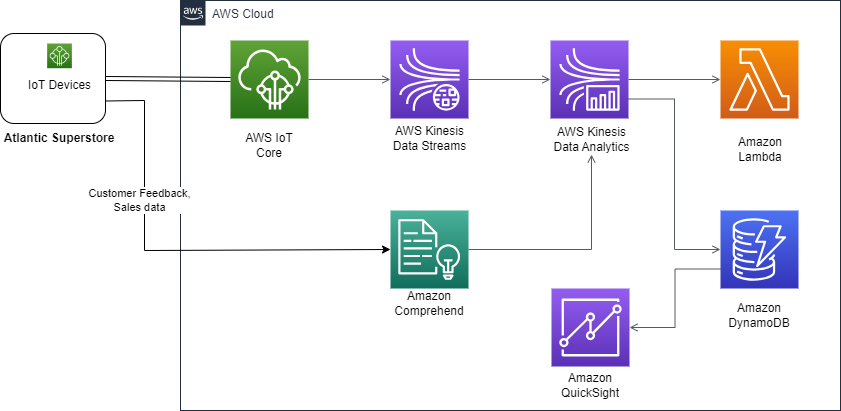
\includegraphics[width=17cm]{PROBLEM 1/Diagram.drawio.png}
    \caption{\textbf{\textit{Smart Inventory Management Architecture at Atlantic Superstore using AWS Services (Created using: draw.io [23])}}}
    \label{fig:aws-arch-diag}
\end{figure}
\begin{enumerate}
    \item \textbf{IoT Devices}: These devices are strategically placed on shelves and equipped with sensors to detect product movement and measure stock levels.
    \item \textbf{AWS IoT Core}: The IoT devices securely connect and transmit data to AWS Kinesis Data Streams, ensuring smooth communication with the cloud.[14]
    \item \textbf{AWS Kinesis Data Streams}: This service captures and streams real-time data from the IoT devices, including product IDs, timestamps, stock levels, and sales data.[15]
    \item \textbf{AWS Kinesis Data Analytics}: The streaming data is processed and analyzed in real-time to forecast demand, identify trending products, and detect potential stock shortages. It also triggers Amazon Lambda functions for automatic reordering and anomaly detection.[16]
    \item \textbf{Amazon Lambda}: Lambda functions automatically trigger reordering processes for low-stock items and flag any irregularities in stock movements.[17]
    \item \textbf{Amazon Comprehend}: This service is used for sentiment analysis, integrating customer feedback with sales data to understand customer preferences and optimize inventory accordingly.[18]
    \item \textbf{Amazon DynamoDB}: The analyzed data is stored in DynamoDB, a NoSQL database, offering fast and scalable access to historical inventory data.[19]
    \item \textbf{Amazon QuickSight}: The data in DynamoDB is visualized and analyzed through QuickSight, enabling the store to create interactive dashboards and gain real-time insights into stock levels, popular products, and inventory performance.[20]
\end{enumerate}



\newpage

\comment{
\chapter*{Revision History}

\begin{center}
    \begin{tabular}{|c|c|c|c|}
        \hline
	    Date & Version & Description & Author\\
        \hline
	     04-Mar-2021 & 1.0 & Interaction Diagram Document - Initial Release. & All\\
        \hline
	    %31 & 32 & 33 & 34\\
        % \hline
    \end{tabular}
\end{center}



\newpage
\tableofcontents
}

\comment{
\chapter{Interaction Diagram}
\begin{figure}[htp]
    \centering
    \includegraphics[width=17.5cm]{04 - Interaction Diagram/Quiz Application-2.png}
    \caption{\textbf{\textit{Login functionality - Interaction diagram}}}
    \label{fig:my_label}
\end{figure}

\begin{figure}[htp]
    \centering
    \includegraphics[width=17.5cm]{04 - Interaction Diagram/Quiz Application-1.png}
    \caption{\textbf{\textit{Quiz Application - Interaction diagram }}}
    \label{fig:my_label}
\end{figure}
}